\section{NLP-based Configuration Completion}

We leverage the regularity of configurations to design an intelligent
configuration completion engine.

According to Hindle et al.~\cite{naturalness}, regularities in bodies of texts
can be easily exploited by natural language processing (NLP) techniques.
Hence, we use n-grams, ranked on the basis of likelihood estimators, to predict
the next token(s) in a configuration.
%Inspired by them, we decided to use N-grams as a basis of our model. This
%effectively makes all router configuration histories a part of the search
%space for our model. 

Prior to building the model, we employ a networking-specific optimization
inspired by our observation that IP prefixes are not common between devices
Section~\ref{sec:similarity}: we replace these tokens with generic {\tt PREFIX}
tokens. As we shown in Section~\ref{sec:results}, this allows us to accurately
predicate the next token in configuration statements involving prefixes.

%In particular, we use an
%n-gram model to generate predictions using likelihood estimators to score our
%n-grams. In particular, we made use of bigrams and trigrams, the latter of
%which performed consistently better. We preprocessed the data and added
%placeholders for certain tokens like IP addresses, subnet masks, and interface
%names

\begin{figure}
	\centering
	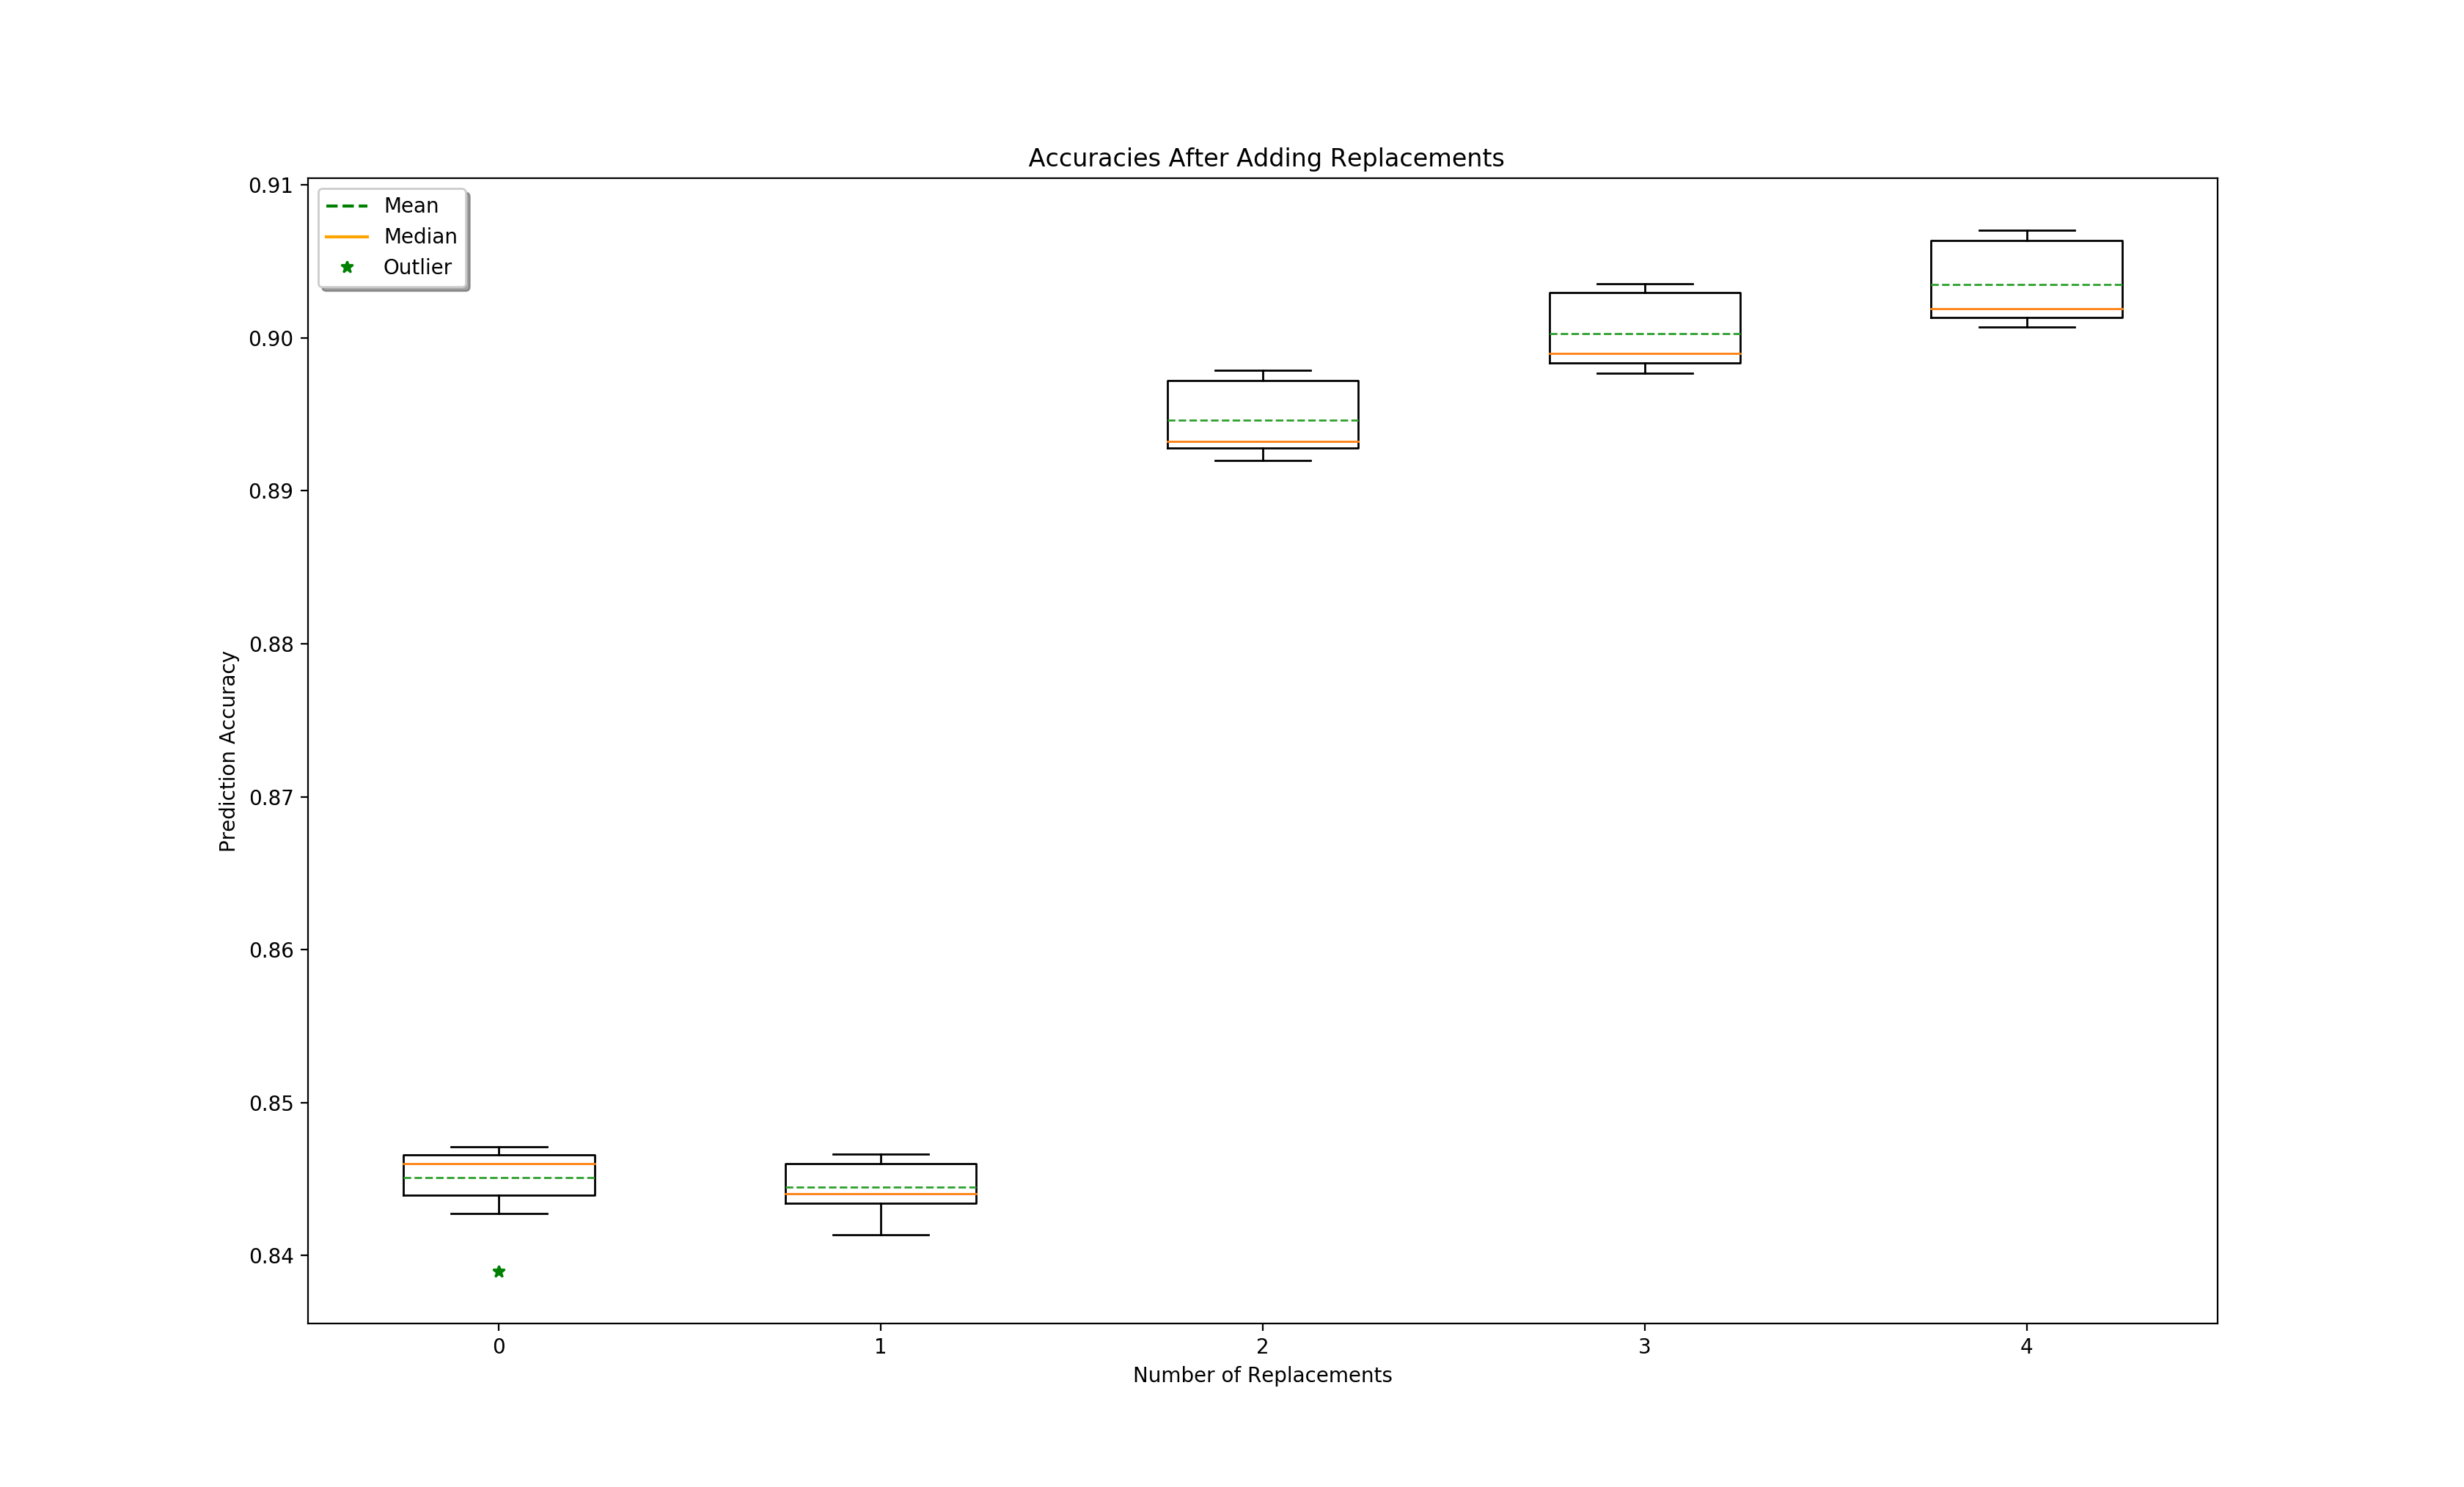
\includegraphics[width=\columnwidth]{replacement_analysis.png}
	\caption{Accuracy increase as we utilize placeholders to replace noisy tokens}
    \label{fig:replacement_analysis}
\end{figure}

\subsection{Preliminary Results}

We applied our framework to configurations of core, border, and distribution routers from three large university networks. Table~\ref{tab:dataset} summaries key characteristics of these configurations. All of the devices are Cisco devices. To test the accuracy of our model, we perform Leave One Out (LOO) Cross Validation. This form of cross validation involves using one observation as the validation set and the remaining observations as the training set. Our program will "walk through" rebuilding a test configuration (A), starting from the first keyword. At every step, we invoke our n-gram model to predict a token using n-1 tokens that came before it. We then compare our predictions against the actual tokens in the test configuration. A prediction is marked as successful when the correct token lies within the top three results generated by the model. Our initial analyses showed that the engine was trying to predict what the user would enter after a complete configuration statement. This greatly affected our accuracies, and thus we altered our model to only suggest tokens that appear on the same line. The table below and (Figure~\ref{fig:config_sizes}) give some statistics about the configurations.

\begin{table}
    \small
    \begin{tabular}{ | p{1.5cm} | p{1.5cm}| p{2cm} |  p{1.5cm} |} 
    \hline
    University & Number of Configurations & Total Number of Lines & Average Number of Lines \\ \hline
    A & 35 & 73000 & 2100 \\  \hline
    B & 26 & 61000 & 2300 \\ \hline
    C & 24 & 67000 & 2800 \\  \hline
    \end{tabular}
    \caption{Configurations used in our evaluation}
    \label{tab:datasets}
\end{table}

\begin{figure}
	\centering
	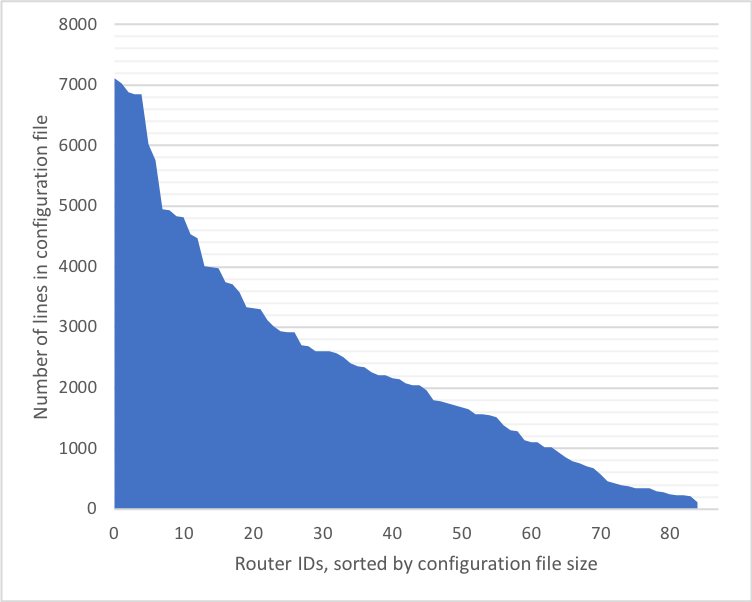
\includegraphics[width=\columnwidth]{config_sizes.png}
	\caption{Size distribution of all configuration files}
    \label{fig:uni_analysis}
\end{figure}

Next, we analyzed the effects of sampling more configuration in time (Figure~\ref{fig:monthly_analysis}), which did not seem to have a statistically relevant effect on our accuracies. We also varied the number of devices considered for our training set (Figure~\ref{fig:device_analysis}). This helped us assess our model's performance when we considered devices with different roles. Additionally, our analyses showed that our preprocessing helped reduce a significant amount of noise from the data, where we saw a 5\% increase in accuracy through placeholders alone. The majority of this increase came through generalizing IP addresses and subnet masks.\\

\begin{figure}
	\centering
	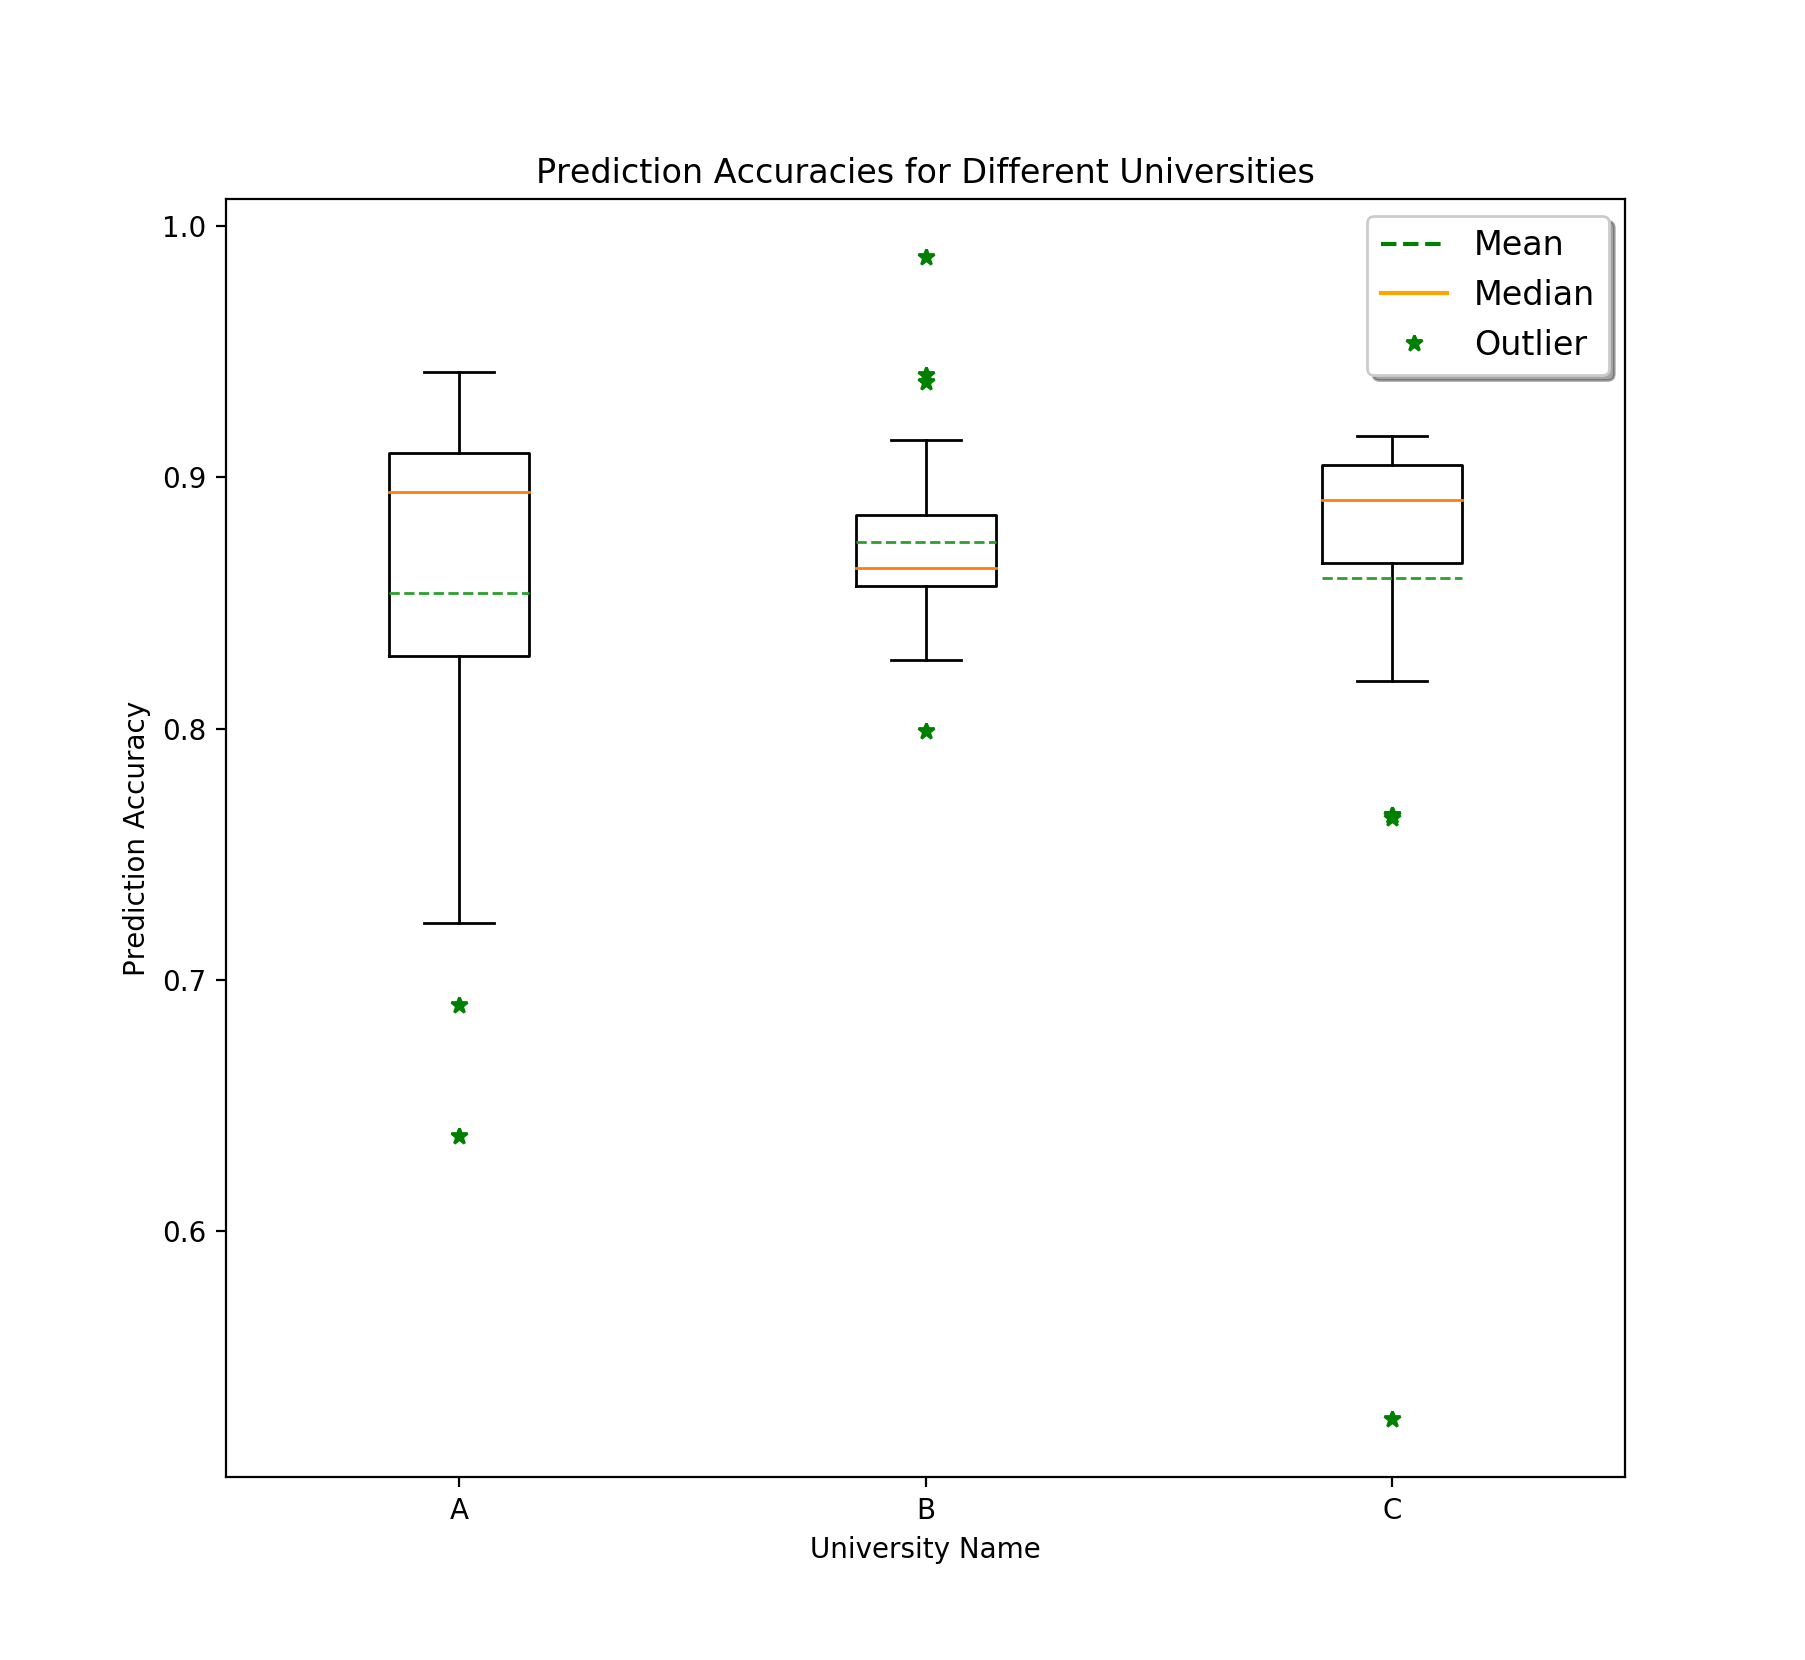
\includegraphics[width=\columnwidth]{uni_analysis.png}
	\caption{Some universities may have routers for different roles, causing more outliers.}
    \label{fig:uni_analysis}
\end{figure}

\begin{figure}
	\centering
	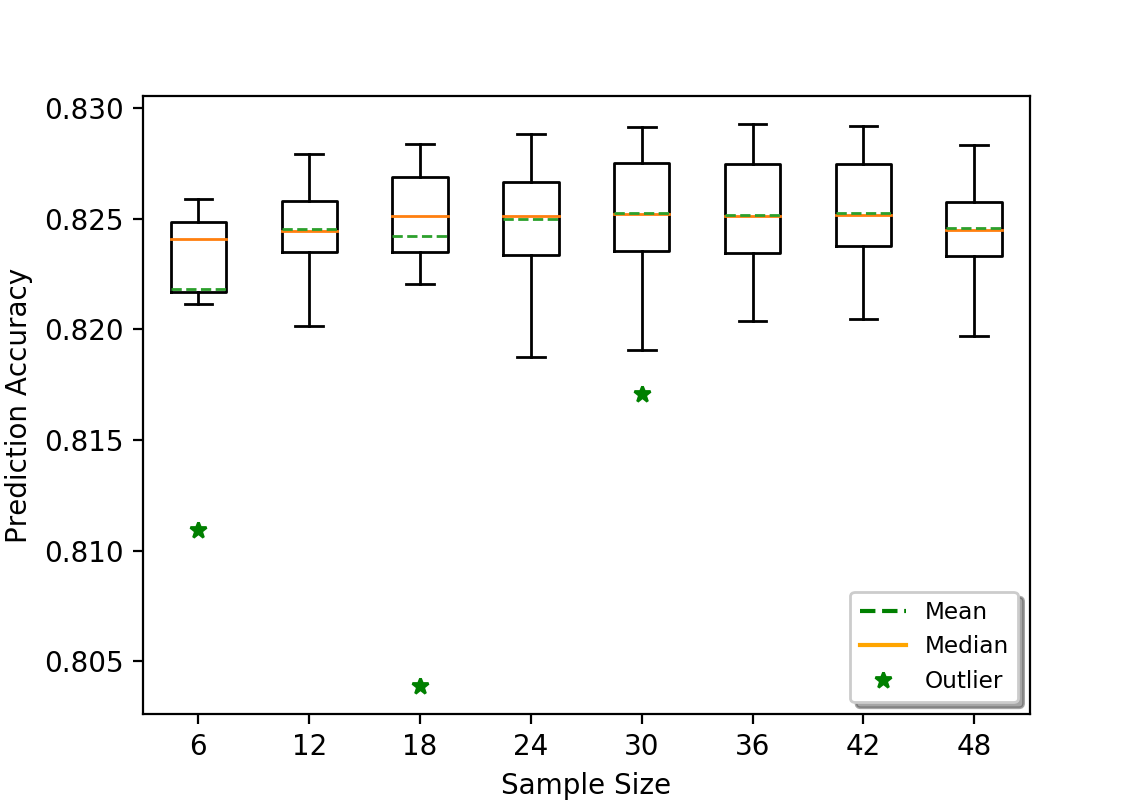
\includegraphics[width=\columnwidth]{monthly_analysis.png}
	\caption{We can achieve the same accuracies by using fewer snapshots in time. Note the small y-axis scale.}
    \label{fig:umn_analysis}
\end{figure}

\begin{figure}
	\centering
	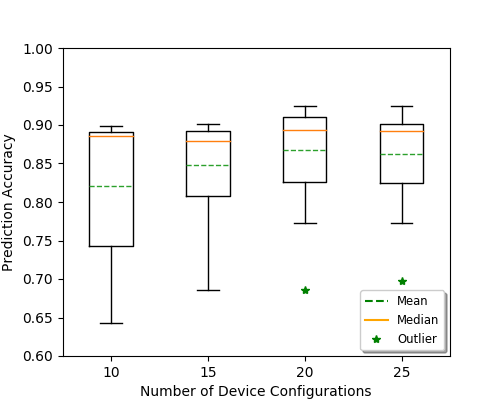
\includegraphics[width=\columnwidth]{device_analysis.png}
	\caption{Accuracies generally increase as more devices are considered, until a saturation point is reached after which the types of devices being added start playing a more important role}
    \label{fig:umn_analysis}
\end{figure}

\section{Future Work}

Our analyses help direct our attention towards areas of improvements for the model. The variance seen in our device analysis suggests that having different models for router of different "roles" could help improve prediction accuracies. Additionally, we plan on exploring the possibility of using larger n-grams to suggest complete statements. Lastly, we hope to evaluate our model against the current state of the art: tab-completion in CLIs on modern routers.
